% TODO:
% - 

%%%%%%%%%%%%%%%%%%%%%%%%%%%%%%%%%%%%%%%%%%%%%%%%%%%%
% documentclss
\documentclass[]{beamer}
%\documentclass[handout]{beamer} %Drucker Version


%%%%%%%%%%%%%%%%%%%%%%%%%%%%%%%%%%%%%%%%%%%%%%%%%%%%
% packages

\usepackage[utf8]{inputenc}
\usepackage[ngerman]{babel}
\usepackage[T1]{fontenc}

\usepackage{setspace}
\usepackage{microtype}
\usepackage{lmodern}

\usepackage{graphicx}
\graphicspath{{images/}}


\hypersetup{
  pdftex,
  bookmarks, bookmarksopen, bookmarksopenlevel=1, bookmarksnumbered=true,
  pdfpagemode={UseNone},
  pdfpagelayout={SinglePage},
  plainpages=false,
  pdfkeywords={Robuste Systeme, ISO 26262},
  pdfsubject={Robuste Systeme - ISO 26262},
  pdftitle={Robuste Systeme - ISO 26262},
  pdfauthor={Martin Wichmann}
}

\usepackage{booktabs}
\usepackage{multirow}

\usetheme{Warsaw}



\AtBeginSection[]
{
   \begin{frame}
        \frametitle{Inhaltsübersicht}
        \tableofcontents[currentsection,currentsubsection]
   \end{frame}
}



%%%%%%%%%%%%%%%%%%%%%%%%%%%%%%%%%%%%%%%%%%%%%%%%%%%%
% Title
\author{Martin Wichmann}
\title{ISO 26262}
\date{\today}
\institute{Ostfalia Hochschule für angewandte Wissenschaften}




%%%%%%%%%%%%%%%%%%%%%%%%%%%%%%%%%%%%%%%%%%%%%%%%%%%%
% begin document
\begin{document}

\begin{frame}
\maketitle
\end{frame}


\begin{frame}
\frametitle{Inhaltsübersicht}
\tableofcontents
\end{frame}





%%%%%%%%%%%%%%%%%%%%%%%%%%%%%%%%%%%%%%%%%%%%%%%%%%%%%%%%%%%%%%%%%%%5
% Einleitung
\section{Einleitung}
\label{sec:einleitung}

\begin{frame}
\frametitle{Information zu Ausarbeitung und Präsentation}
\begin{itemize}
    \item ISO Norm nicht verfügbar
    \item Kaum Literatur vorhanden
    \item Ausarbeitung und Präsentation basieren fast komplett auf \cite{1}
    \begin{itemize}
        \item Befasst sich vor allem mit DIN 61508
    \end{itemize}
    \item Bilder sind aus Buch übernommen
\end{itemize}
\end{frame}


\begin{frame}
\frametitle{Funktionale Sicherheit}

\begin{itemize}
    \item Methodischer Ansatz für Sicherheit
    \item Beschreibt feste Anforderungen und Vorgehensweisen
    \item Sicherheit soll möglichst Objektiv werden
    \item Funktionale Sicherheit lediglich allgemeines Konzept
    \item Implementationen zum Beispiel:
    \begin{itemize}
        \item DIN 61508 (E/E/PES)
        \item ISO 26262 (Personenkraftwagen)
        \item DIN 60601 (Medizin-Geräte)
    \end{itemize}
\end{itemize}

\end{frame}


\begin{frame}
\frametitle{ISO 26262}

\begin{itemize}
    \item Internationale Norm für Automotive-Bereich
    \item Freigabe: 14. November 2011
    \item Kapitel 10 fehlt noch
    \item Basiert auf DIN 61508 (1998) und erweitert diese
    \begin{itemize}
        \item Serienproduktion
        \item Wartung
        \item Außerbetriebnahme
    \end{itemize}
\end{itemize}

\end{frame}




\begin{frame}
\frametitle{Struktur ISO 26262}

\begin{enumerate}
    \item Vokabular
    \item Management der funktionalen Sicherheit
    \item Konzept-Phase
    \item Produktentwicklung: Systemebene
    \item Produktentwicklung: Hardwareebene
    \item Produktentwicklung: Softwareebene
    \item Produktion, Betrieb und Außerbetriebnahme
    \item Unterstützende Prozesse
    \item ASIL- und sicherheitsorientierte Analysen
    \item Guideline
\end{enumerate}

\end{frame}



%%%%%%%%%%%%%%%%%%%%%%%%%%%%%%%%%%%%%%%%%%%%%%%%%%%%%%%%%%%%%%%%%%%5
% Sicherheitslebenszyklus und Planung
\section{Sicherheitslebenszyklus und Planung}
\label{sec:Sicherheitslebenszyklus_Planung}

\begin{frame}
\frametitle{Überblick Sicherheitslebenszyklus}
\begin{figure}
   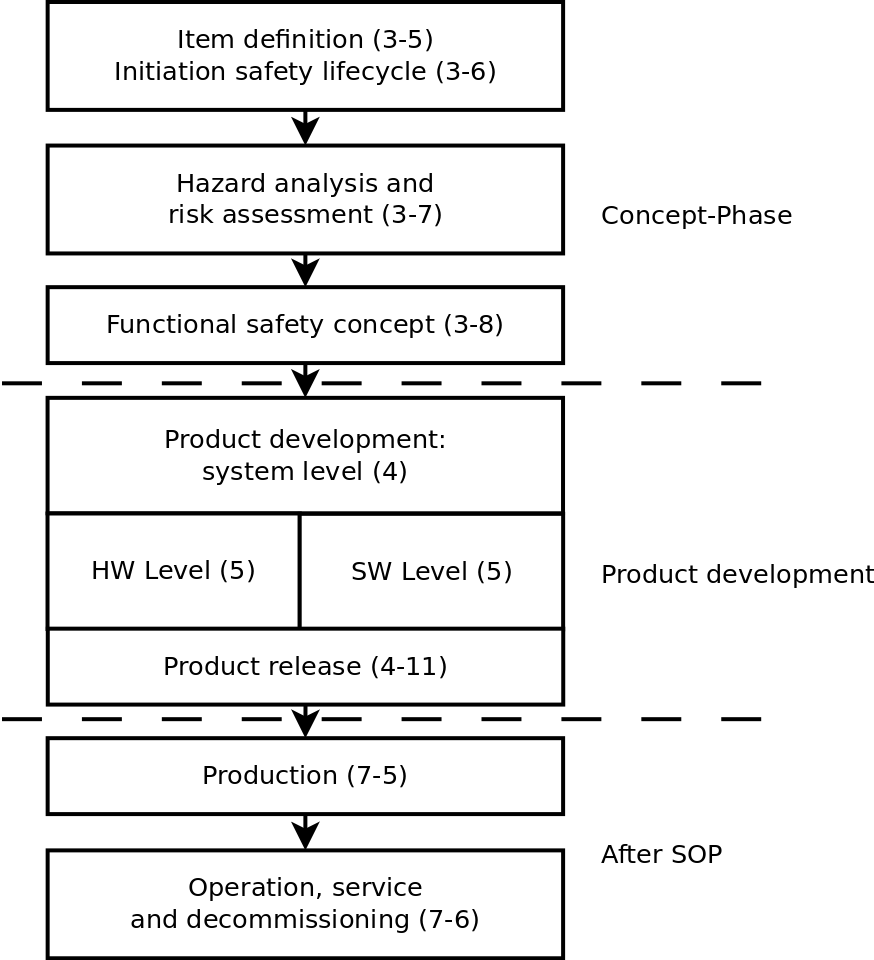
\includegraphics[width=6cm]{Abb_6_1}
\end{figure}
\end{frame}


\begin{frame}
\frametitle{Management der funktionalen Sicherheit}

\begin{itemize}
    \item asd
\end{itemize}

\end{frame}

\begin{frame}
\frametitle{Gefährdungsanalyse und Risikoeinschätzung}

\begin{itemize}
    \item asd
\end{itemize}

\end{frame}



%%%%%%%%%%%%%%%%%%%%%%%%%%%%%%%%%%%%%%%%%%%%%%%%%%%%%%%%%%%%%%%%%%%5
% Produktentwicklung
\section{Produktentwicklung}
\label{sec:Produktentwicklung}

\begin{frame}
\frametitle{Produktentwicklung}

\begin{itemize}
    \item asd
\end{itemize}

\end{frame}





\subsection{Systemebene}
\begin{frame}
\frametitle{Systemebene Überblick}

\begin{itemize}
    \item asd
\end{itemize}

\end{frame}

\begin{frame}
\frametitle{Systemebene Methoden}

\begin{itemize}
    \item asd
\end{itemize}

\end{frame}





\subsection{Hardware}
\begin{frame}
\frametitle{Hardware Überblick}

\begin{itemize}
    \item asd
\end{itemize}

\end{frame}

\begin{frame}
\frametitle{Hardware Fehlerarten}

\begin{itemize}
    \item asd
\end{itemize}

\end{frame}

\begin{frame}
\frametitle{Hardware Metriken}

\begin{itemize}
    \item asd
\end{itemize}

\end{frame}

\begin{frame}
\frametitle{Hardware Methoden}

\begin{itemize}
    \item asd
\end{itemize}

\end{frame}




\subsection{Software}

\begin{frame}
\frametitle{Software Überblick}

\begin{itemize}
    \item asd
\end{itemize}

\end{frame}

\begin{frame}
\frametitle{Software Methoden}

\begin{itemize}
    \item asd
\end{itemize}

\end{frame}



%%%%%%%%%%%%%%%%%%%%%%%%%%%%%%%%%%%%%%%%%%%%%%%%%%%%%%%%%%%%%%%%%%%5
% Fazit
\section{Fazit}
\label{sec:Fazit}

\begin{frame}
\frametitle{Fazit}

\begin{itemize}
    \item asd
\end{itemize}

\end{frame}








%%%%%%%%%%%%%%%%%%%%%%%%%%%%%%%%%%%%%%%%%%%%%%%%%%%%%%%%%%%%%%%%%%%5
% Literaturangaben
\appendix
\section*{Literatur}
\label{sec:Literatur}

\begin{frame}
\begin{thebibliography}{10}

\bibitem[1]{1} \textsc{Peter Löw, Roland Pabst, Erwin Petry}: {\em Funktionale Sicherheit in der Praxis.} dpunkt.verlag, 2010.

\end{thebibliography}
\end{frame}





















\end{document}










